\chapter{Environnement de travail}
\label{sec:EnvironnementDeTravail}
L'objectif de ce chapitre consiste à expliciter tous les éléments relatifs à l'environnement logiciel sur lequel j'ai travaillé pour réaliser cette application. Il s'agit donc des logiciels, langages, frameworks, et motifs d'architecture auxquels j'ai fait recours tout au long du processus de mise en œuvre de ma solution.
\section{Gestion du projet}
Dans cette section, je présente la méthodologie de travail et le logiciel de gestion de projet que j'ai utilisé pour déclencher, organiser et gérer le travail sur ma solution.
\subsection{Méthodologie de travail}
C'est la manière de mener un processus de développement. Il s’agit d’une démarche, un ensemble d’étapes ou procédures à mettre en œuvre dans une logique méthodologique, accompagnés d’outils et de techniques. L'utilisation d'une méthode est incontournable dans l'entreprise de tout projet, particulièrement dans la réalisation de projets informatiques. Dans ce cas-ci, les méthodes utilisées sont des méthodes d'analyse et de conception qui ont pour but la formalisation des étapes préliminaires au développement de systèmes logiciels, en d'autres termes : analyse, modélisation et conception. \newline
L'urgence de l'utilisation de ces méthodes trouve son explication dans un certain nombre de facteurs :
\begin{enumerate}
	\item De nombreux échecs de projets informatiques dans le passé dus à un manque d'organisation, ou une non satisfaction des besoins ;
	\item La révolution de l'industrie logicielle engendrée par les échecs informatiques et qui introduit de nouveaux facteurs de validation de la qualité logicielle : le génie logiciel ;
	\item Les nombreuses exigences liées au coût, aux délais et à la complexité des projets informatiques.
\end{enumerate}

L'utilisation de méthodes de développement de logiciels permet ainsi l'élaboration de systèmes informatiques de manière fiable et viable tout en répondant à l'ensemble des exigences du client et du génie logiciel.
\newline \newline
Il existe plusieurs méthodes de développement informatique. L’on distingue deux approches : l’approche traditionnelle et l’approche agile. Les deux approches se distinguent essentiellement dans la manière de décomposer le projet. Les méthodes cartésiennes ou fonctionnelles ou encore traditionnelles se sont imposées les premières.
\subsubsection{L'approche traditionnelle}
Cette approche s’inspire directement de l’architecture des ordinateurs. Les méthodes traditionnelles prônent une démarche strictement planifiée avec une séquence d’activités bien définie. La succession des activités et le planning doivent être clairement respectés et aucun changement n’est permis. Il est attendu du client une spécification des besoins globale, détaillée, claire, précise et validée en entrée. Ainsi, tout doit être prévisible, du début du projet à la livraison du produit, d’où l’appellation de méthodes prédictives. \newline
Selon le planning adopté, les méthodes cartésiennes proposent plusieurs modèles d’exécution des activités du projet :
\begin{enumerate}
	\item Le \textbf{modèle en cascade} : dans ce modèle, le processus de développement est découpé séquentiellement et de façon linéaire selon les activités intrinsèques du cycle de vie du développement logiciel : l’analyse, la conception, le codage et les tests. Le plan de déroulement des phases (planification prédictive) est élaboré en tout début de processus. Le passage à une phase donnée n’est fait que si le résultat de la phase précédente a été validé et jugé satisfaisant par le client et les utilisateurs.
	\item Le \textbf{modèle en V} : Le cycle en V est à la base de tout développement logiciel, il en représente les activités intrinsèques. Il tient d'avantage compte de la réalité que le modèle en cascade, le processus de développement n’est pas réduit à un enchainement de tâches séquentielles. Le modèle en V permet d’anticiper sur les phases ultérieures de développement du produit en particulier les plans de test de qualifications et de performance.
\end{enumerate}
Parmi les méthodes traditionnelles, nous pouvons citer : SADT, CORIG, …
\subsubsection{L'approche agile}
Cette approche est définie par les concepts suivants : la simplicité, la légèreté, la souplesse, un lien fort avec le client. C’est dans cette optique que certains apparentent le développement agile aux notions de flexibilité, de rétroaction et d’adaptation au changement rapide et continu.
\newline
Une méthode agile est une approche itérative et incrémentale, qui est menée dans un esprit collaboratif avec juste ce qu’il faut de formalisme. Elle génère un produit de haute qualité tout en prenant en compte l’évolution des besoins des clients et en anticipant sur les risques. Il y’a continuellement des aller et retour avec le client. L’application logicielle est livrée par version incrémentale. Les versions successives sont aussi fiables que le livrable final en termes de tests et de validation. En quelque sorte le processus est déroulé comme un enchaînement de « mini-cascades ». A chaque nouvelle itération, l’ensemble de l’architecture et de la conception logicielle est reconsidéré, le code est retravaillé.
\newline
Les méthodes agiles aspirent donc à améliorer la réactivité et l’adaptabilité des sociétés de logiciels et constituent un moyen de survie dans un environnement instable en s’accompagnant des valeurs suivantes :
\begin{enumerate}
	\item Les individus et les interactions plutôt que les processus et les outils;
	\item L’application fonctionnelle plutôt que la documentation compréhensive;
	\item La collaboration avec le client plutôt que la négociation des contrats;
	\item La réponse au changement plutôt que le suivi d’un plan.
	\newline
\end{enumerate}
L’agilité comprend plusieurs courants de pensée qui ont conduits à des méthodes différentes, reposant sur les mêmes concepts mais présentant des singularités. Les méthodes Scrum, Kanban, et XP (eXtreme Programming) sont des exemples de ces méthodes.
\newline\newline

\textbf{La méthode SCRUM}
\newline
\textbf{Scrum} est une méthode agile de gestion de projet qui permet de produire la plus grande valeur métier dans la durée la plus courte. Elle a pour objectif d’améliorer la cohésion de l’équipe et la rapidité du processus de développement. Le nom Scrum renvoie à une pratique généralement connue au rugby signifiant la « mêlée ». \newline
Cette méthode qualifie un ensemble de rôles, d’instruments de gestion et de pratiques managériales favorisant un environnement basé sur la transparence, l’inspection, le suivi et l’adaptation. Le cycle de vie d’un projet Scrum peut être découpé en trois parties :
\begin{enumerate}
	\item Phase d'\textbf{initiation ou démarrage} : il s’agit d’une phase linéaire où l’on définit le périmètre fonctionnel du système et la liste des fonctionnalités (\textbf{Backlog}) agencées par ordre de priorité, d’effort, de complexité et de risque. C’est aussi à ce niveau que l’architecture est définie.
	
	\item Phase de \textbf{développement} est un processus empirique : le projet est découpé en cycles itératifs d’une durée de deux semaines ou \textbf{sprints}. Chaque sprint regroupe une ou plusieurs fonctionnalités du Backlog. Tout au long de cette phase, le travail réalisé est mesuré et contrôlé et une amélioration constante du prototype est faite.
	
	\item Phase de \textbf{Clôtures} est une phase linéaire de gestion de la livraison du produit final.
\end{enumerate}
La figure \ref{Scrum} montre l’articulation générale de Scrum. \newline
\begin{figure}[h]
	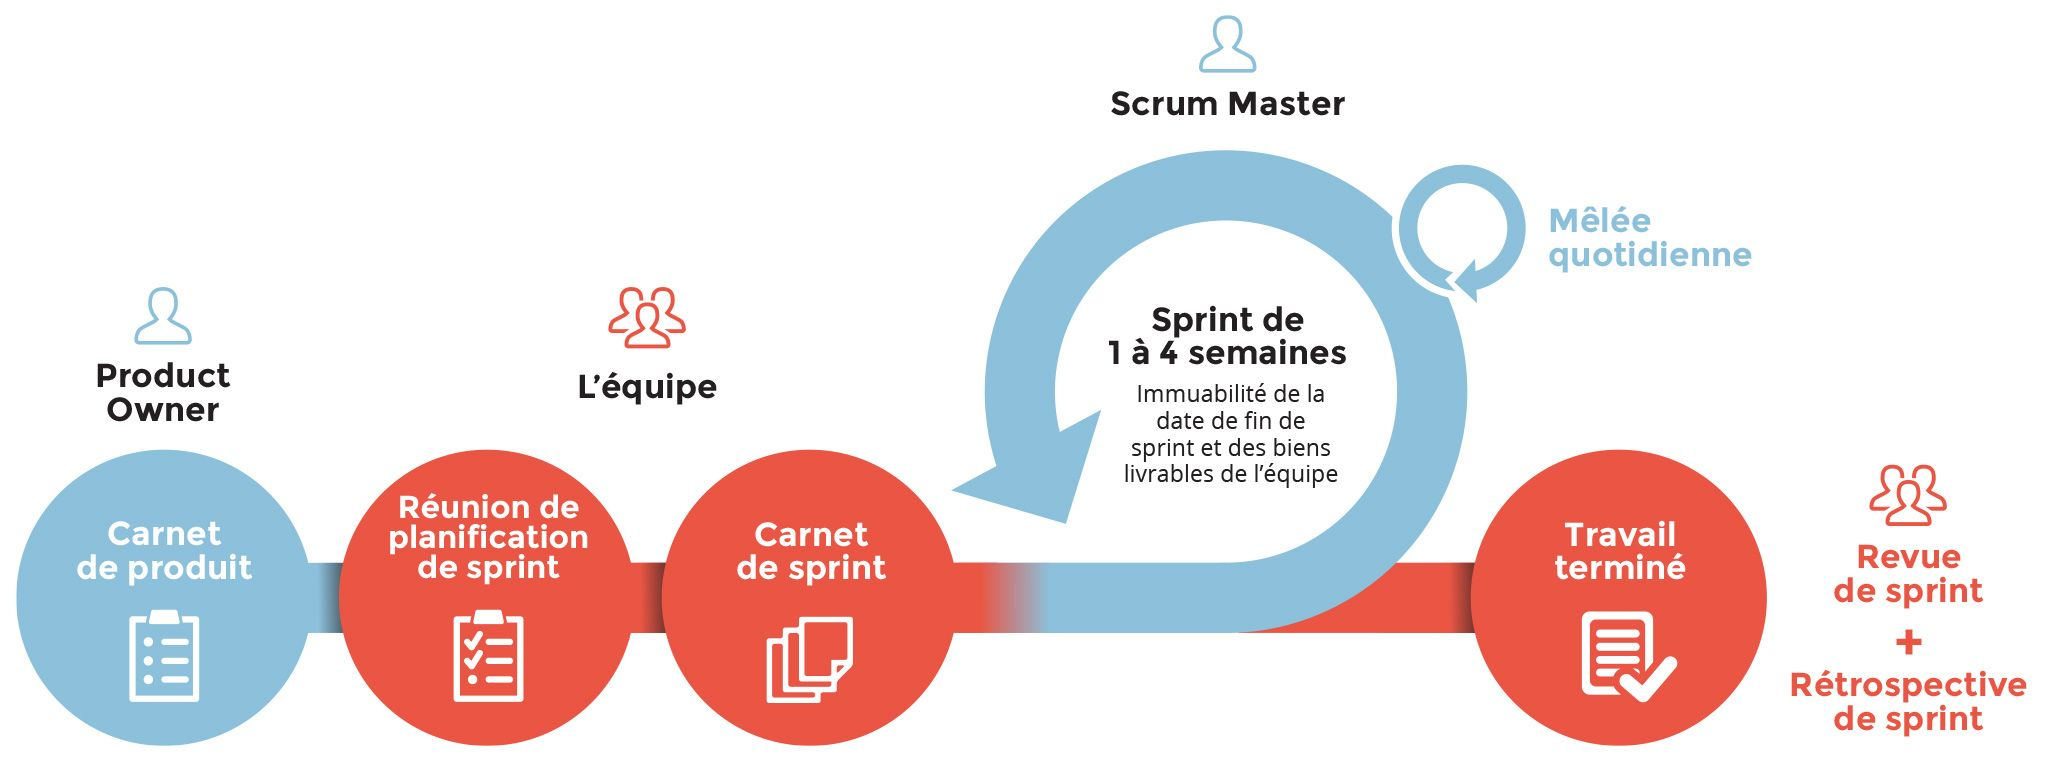
\includegraphics[width=15cm, height=5cm]{/home/mohamed/mes_fichier/CADORIM/LaTeX/pfe/Template LaTeX/Images/scrum1.jpeg}
	\centering
	\caption{Articulation générale de la méthode Scrum}
	\label{Scrum}
\end{figure}
Les responsabilités managériales sont réparties sur trois rôles fondamentaux :
\begin{enumerate}
	\item \textbf{Scrum Master}
	\item \textbf{Product Owner}
	\item \textbf{Équipe Scrum}
	\newline
\end{enumerate}
Les artéfacts et pratiques de Scrum
\begin{enumerate}
	\item \textbf{Product Backlog} : état courant des tâches à accomplir;
	\item \textbf{Sprint} : itération de deux semaines;
	\item \textbf{Effort-Estimation} : permanente sur les entrées du Backlog;
	\item \textbf{Sprint Backlog} : Product Backlog limité au sprint en cours;
	\item \textbf{Daily Scrum Meeting} : ce qui a été fait, ce qui reste à faire;
	\item \textbf{Sprint Review Meeting} : Présentation des résultats du Sprint. \ref{Scrum}
	\newline \newline \newline
\end{enumerate}
\textbf{SCRUM contre KANBAN}
\newline
Scrum est plus prescriptif que Kanban, qui évite de définir les rôles et les équipes et qui n’a pas de structure formelle de réunions. Kanban ne prescrit pas non plus d’itérations – bien qu’elles puissent être incorporées si vous le souhaitez. \newline
Les techniques de visualisation des processus de Kanban le rendent idéal pour les équipes colocalisées qui travaillent sur un backlog d’éléments sujets à des changements fréquents (par exemple, Kanban est souvent utilisé par les équipes de support). \newline
Le tableau Kanban est cependant souvent adopté par les équipes Scrum sous la forme d’un tableau de tâches et est utilisé pour suivre la progression tout au long d’un sprint. \newline
La limite de la règle Work In Progress dans Kanban la rend également adaptée aux équipes ayant des ressources limitées ou lorsque l’entrée de chaque membre est requise sur chaque élément. Cela pourrait s’appliquer, par exemple, à une équipe de communication au sein d’une grande organisation. \newline
Alors que Scrum limite la quantité de travail dans chaque sprint, la charge de travail est déterminée par l’estimation relative de la taille de chaque histoire (en points) et est approuvée par l’équipe Scrum à chaque session de planification. \newline
Alors qu’une équipe Kanban suit le « temps de cycle » et optimise les délais d’exécution aussi courts et prévisibles que possible, une équipe Scrum vise à améliorer son rendement sur les sprints successifs et à améliorer la « vélocité » de l’équipe (le nombre de points d’estimation relatifs complétés dans un sprint). Cela rend sans doute Scrum plus adapté à la mise à l’échelle – il semble certainement plus familier et prévisible, ce qui peut être rassurant pour les grandes organisations. \newline\newline
\textbf{SCRUM contre XP}
\newline
Dans Scrum, les équipes et les réunions sont assez gravées dans le marbre \footnote{Dans l’antiquité, les engagements pour la constructions de bâtiments importants étaient gravés sur des plaques de marbre (Athènes : arsenal du Pirée, Delphes). Les travaux s’étendant sur de nombreuses années, on ne pouvait faire confiance aux tablettes de cire ou aux papyrus. Sur ces plaques, on définissait par exemple la grandeur du bâtiment ou le montant des amendes pour les retards. Ce qui n’était pas « gravé dans le marbre » n’était donc pas contractuel. Voir le lien \href{https://fr.wiktionary.org/wiki/graver_dans_le_marbre}{https://fr.wiktionary.org/wiki/graver-dans-le-marbre}} alors que la question de savoir comment le travail est réellement fait est laissée aux équipes pour décider elles-mêmes. XP, d’autre part, est livré avec un ensemble de pratiques de base qui pourraient sembler accablantes pour le débutant Agile. \newline
On pourrait dire que Scrum est une méthodologie, qui est plus concernée par la productivité tandis que XP est plus préoccupé par l’ingénierie. \newline
La valeur que les pratiques XP peuvent ajouter est incontestable et de nombreuses organisations qui utilisent Scrum adoptent la programmation par paires, le développement piloté par les tests et le refactoring comme des pratiques qui améliorent la qualité, accélèrent le processus de publication et / ou réduisent le besoin de revoir le travail en raison de la dette technique. \newline
Outre les itérations plus courtes, d’autres éléments importants qui différencient XP de Scrum sont les suivants :
\begin{enumerate}
	\item Les équipes XP travaillent sur des éléments dans un ordre de priorité strict alors qu’une équipe Scrum ne s’attaque pas nécessairement à chaque élément dans l’ordre de priorité une fois dans le sprint;
	\item Les équipes XP peuvent intégrer de nouveaux éléments de travail dans une itération et changer d’éléments de taille équivalente (tant qu’ils n’ont pas été démarrés) si le client décide d’une nouvelle priorité.
	
	%%%%%%%%%%%%%%%%%%%%%%%%%%%%%%%%%%%%%%%%%%%%%%%%%%%%%%%%%%%%%%%%%%%%%%%%%%%%%%%%%%%%%%%%%%%%%%
\end{enumerate}
En termes de similitudes, le rôle du client dans XP est très similaire à celui du Product Owner dans Scrum – en ce sens qu’ils aident à écrire des user stories, à les hiérarchiser et sont toujours disponibles pour les développeurs – bien que moins bien définis. \newline
Scrum et XP imposent tous deux une réunion debout quotidienne. Bien que les deux soulignent l’importance de la co-localisation, seul XP le rend décisif. Voir le site \href{https://manifesto.co.uk/kanban-vs-scrum-vs-xp-an-agile-comparison/}{https://manifesto.co.uk/kanban-vs-scrum-vs-xp-an-agile-comparison/}.


\subsection{Logiciel de gestion du projet : Trello}
Trello est un outil de gestion de projet en ligne, lancé en septembre 2011 et inspiré par la méthode Kanban. Il repose sur une organisation des projets en planches listant des cartes, chacune représentant des tâches. Les cartes sont assignables à des utilisateurs et sont mobiles d'une planche à l'autre, traduisant leur avancement. Pour en savoir plus, veillez visiter le lien \href{https://fr.wikipedia.org/wiki/Trello}{https://fr.wikipedia.org/wiki/Trello}.

\section{Conception}
Dans cette section, je présente le langage et le logiciel de modélisation que j'ai utilisé pour concevoir notre solution.

\subsection{Langage de modélisation : UML}
UML est un langage de modélisation orientée objet permettant aux développeurs de modéliser un système d’information en considérant plusieurs vues chacune reflétant un aspect comportemental \footnote{Diagramme de cas d’utilisation, diagramme d’activité, diagramme de séquence, diagramme d’interaction, etc.} ou structurel \footnote{Diagramme de classe, diagramme de composants, diagramme de déploiement, diagramme de structure composite, etc.} du système.
\newline
En effet, nous avons opté pour UML au détriment de la MERISE car nous avons besoin
d’une approche de conception prenant en considération l’aspect orienté objet pour :
\begin{enumerate}
	\item Pouvoir mettre le focus sur le rôle temporel des instances d’objets lors de déclenchement desactions (à travers le diagramme de séquence) ;
	\item Faciliter par la suite la génération des classes DAO à partir du diagramme de classes.
\end{enumerate}
Certes, UML est très riche en matière de modélisation et propose au total 13 diagrammes chacun fournissant une vision particulière du système à concevoir. Dans notre contexte, je me suis limités à 4 diagrammes explicités sur le tableau \ref{3.1}.

\subsection{Logiciel de modélisation}
Modelio est un logiciel open source et multiplateforme permettant, entre autres, la modélisation UML et Business Process Model and Notation (BPMN). Pour en savoir plus, veuillez visiter le lien \href{https://www.modelio.org/about-modelio/features.html}{https://www.modelio.org/about-modelio/features.html}.
\newline
Sans doute, les logiciels de modélisation UML sont nombreux, à savoir, Visual Paradigm, Eclipse Papyrus, StarUML, PowerDesigner, Umbrello, etc. Vu que les diagrammes UML que nous voulons réaliser sont disponibles dans tous ces logiciels, il n’y avait pas en effet un choix à argumenter car
tous les choix étaient satisfaisants. Mais, de façon subjective, nous pouvons préciser que l’avantage de Modelio dans notre contexte est le fait que je m'y suis	 déjà habitués. Les diagrammes que nous avons réalisés avec Modelio sont ceux mentionnés ci-après.
\newline\newline
\begin{table}[h]
	\begin{tabular}{|m{6cm}|m{10cm}|}
		\hline
		\textbf{Diagramme} & \textbf{Rôle} \\
		\hline
		Diagramme de cas d’utilisation & Présenter les acteurs du système, ses fonctionnalités, les relations entre les acteurs et entre les fonctionnalités. \\
		\hline
		Diagramme d’activité & Déterminer l’enchaînement des différentes étapes qui composent une fonctionnalité du système. \\
		\hline
		Diagramme de séquence & Fournir une vue détaillée du diagramme d’activité en mettant le focus sur l’ordre chronologique et sur les objets crées et les méthodes appelées. \\
		\hline
		Diagramme de classe & Représenter la structure interne du système sous forme de classes et d’interfaces et préciser les différentes relations entre elles. \\
		\hline
		
	\end{tabular}
	\caption{Rôles des diagrammes UML utilisés.}
	\label{3.1}
\end{table}

\section{Implémentation}
Dans cette section, je présente les langages, les logiciels, les frameworks et les motifs d’architecture que j'ai utilisé.

\subsection{Front-end}
\subsubsection{Editeur de texte : VS Code}
VS Code (Visual Studio Code) est un éditeur de code source réalisé par Microsoft pour Windows, Linux et macOS. [9] Les fonctionnalités incluent la prise en charge du débogage, lacoloration syntaxique, la saisie semi-automatique intelligente du code, les extraits de code, la refactorisation du code et Gitintégré. Les utilisateurs peuvent modifier le thème,les raccourcis clavier,les préférences et installer des extensions qui ajoutent des fonctionnalités supplémentaires. Pour en savoir plus, veillez visiter le lien \href{https://en.wikipedia.org/wiki/Visual_Studio_Code}{https://en.wikipedia.org/wiki/VisualStudioCode}.
\subsubsection{Languages}
\begin{table}[h]
	\begin{tabular}{|m{6cm}|m{10cm}|}
		\hline
		\textbf{Langage} & \textbf{Contexte d’utilisation} \\
		\hline
		Dart & Création des applications moible\\
		\hline
		PHP  & Langage de programmation libre, principalement utilisé pour produire des pages Web dynamiques via un serveur HTTP\\
		\hline
		
	\end{tabular}
	\caption{Contexte d’utilisation des différents langages utilisés.}
\end{table}
\subsubsection{Framework : Flutter}
\label{Flutter}
Flutter est un cadre de développement d’applications mobiles open source permettant de développer des applications mobiles natives Andriod et iOS en un seul code.

Flutter a été introduit par Google. La version stable de Flutter est Flutter 1.0 qui a été publiée le 4 décembre 2018. Le ciel est la première application Flutter qui a fonctionné dans l’OS Andriod. \href{https://www.claudebueno.com/technologies/introduction-a-flutter.htm}.
\subsubsection{Framework Web :  Laravel}
\label{Laravel}
Laravel est un framework d'application Web avec une syntaxe expressive et élégante. Nous croyons que le développement doit être une expérience agréable et créative pour être vraiment épanouissante. Laravel tente de simplifier le développement en facilitant les tâches courantes utilisées dans la majorité des projets Web, telles que l'authentification, le routage, les sessions et la mise en cache.

Laravel vise à rendre le processus de développement agréable pour le développeur sans sacrifier les fonctionnalités de l'application. Les développeurs heureux font le meilleur code. À cette fin, nous avons tenté de combiner le meilleur de ce que nous avons vu dans d'autres frameworks Web, y compris des frameworks implémentés dans d'autres langages, tels que Ruby on Rails, ASP.NET MVC et Sinatra.

Laravel est accessible, mais puissant, fournissant des outils puissants nécessaires pour les applications volumineuses et robustes. Une superbe inversion du conteneur de contrôle, un système de migration expressif et une prise en charge des tests unitaires étroitement intégrée vous offrent les outils dont vous avez besoin pour créer n'importe quelle application qui vous est confiée.
\href{https://laravel.com/docs/4.2/introduction#laravel-philosophy}.
\subsubsection{IDE : Android Studio}
Android Studio est l’IDE officiel pour le système d’exploitation Android de Google,construit sur le logiciel IntelliJ IDEA de JetBrainset conçu spécifiquement pour le développement Android. Pour en savoir plus veillez visiter le lien \newline \href{https://en.wikipedia.org/wiki/Android_Studio}{https://en.wikipedia.org/wiki/AndroidStudio}. \newline
Essentiellement, je l'ai utilisé pour lancer l'application sur android.
\subsection{Back-End}
\subsubsection{IDE : Visual Studio}
Microsoft Visual Studio est un IDE de Microsoft. Il est utilisé pour développer des programmes informatiques, ainsi que des sites Web, des applications Web, des services Web et des applications mobiles. Pour en savoir plus, veillez visiter le lien \href{https://en.wikipedia.org/wiki/Microsoft_Visual_Studio}{https://en.wikipedia.org/wiki/MicrosoftVisualStudio}.
\subsubsection{MVC}
\label{3.3.3.1}
L'objectif du motif MVC (Model-View-Controller ou Modèle-Vue-Contrôleur) est un modèle dans la conception de logiciels. Il met l'accent sur la séparation entre la logique métier et l'affichage du logiciel. Cette «séparation des préoccupations» permet une meilleure répartition du travail et une maintenance améliorée. Le tableau ci-dessous en présente une explication.
\newline\newline
\begin{table}[h]
	\begin{tabular}{|m{6cm}|m{10cm}|}
		\hline
		\textbf{Couche logicielle} & \textbf{Rôle} \\
		\hline
		Modèle & Gère les données et la logique métier \\
		\hline
		Vue & Gère la disposition et l'affichage \\
		\hline
		contrôleur & Chemine les commandes des parties "model" et "view" \\
		\hline
	\end{tabular}
	\caption{Rôle des trois couches logicielles du motif MVC.}
\end{table}
\newline La figure ci-dessous explique les moments d'intervention de chaque couche du motif MVC.
\begin{figure}[h]
	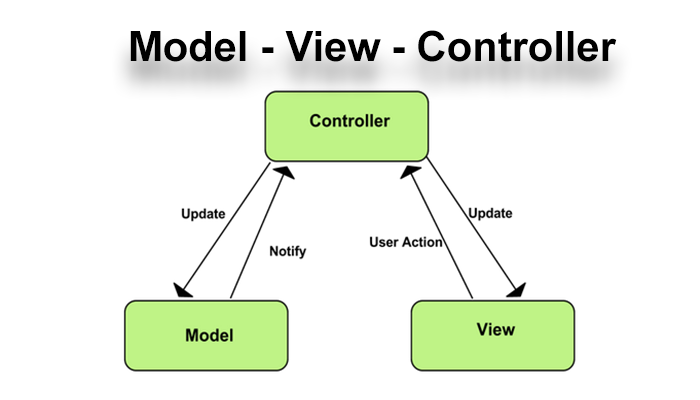
\includegraphics[width=15cm, height=8cm]{/home/mohamed/mes_fichier/CADORIM/LaTeX/pfe/Template LaTeX/Images/mvc2.png}
	\centering
	\caption{Rôle des trois couches logicielles du motif MVC}
\end{figure}
\section{Sécurité}
Dans cette section, je présente les algorithmes et techniques de chiffrement que nous avons
utilisés pour sécuriser davantage l'application.
\subsection{Hachage des mots de passe}